\chapter{Results and Discussion}\label{chap:results}
% Evaluation Criteria:
% - Quality of explanation (written)
% - Support with diagrams, tables and figures
% - Table headings and figure captions
% - Clear axis labels on all figures
% - Figure complexity
% Discussion
% - Quality of explanations (written)
% - Comparison with related work
% - Discussion of implications
% - Discussion of limitations
\section{Overview}
\subsection{Recap}
\draft{Before, ....}
\todo{make quick recap on approach for who starts reading here}

\subsection{What's to come}
\draft{In this Chapter, ...}

\subsection{Note on differences to impl}
\todo{redo subsection titles and structure}
\textbf{Note} that while all code (refer to \secref{impl} for notes on implementation) includes \texttt{additive}, figures in this chapter do not.
This decision was made due to mistaken modeling of the task, which resulted in horrendous accuracy.
7B-sized models all had less than 1\% correct (except for Vicuna with 2.5\%), and even large models had either below 1\% or around 15\% correct (\model{llama2} and \model{falcon}, not the instruct-variant).

Instead of literal extraction, the task should have been modeled as classification task.
This was not redone due to time constraints.


\begin{figure}[!htbp]
    \begin{centering}
        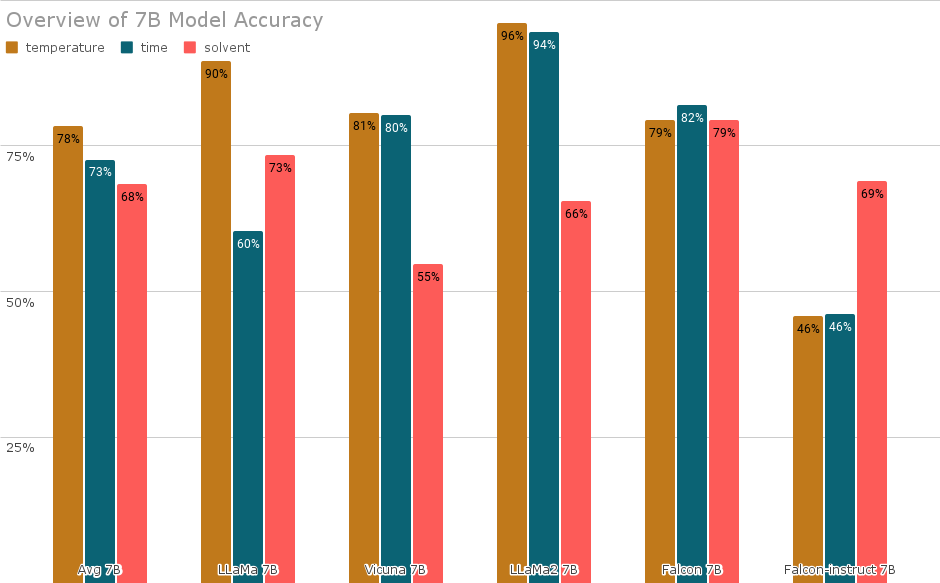
\includegraphics[width=0.9\textwidth]{img/overview_7b_accuracy}
        \caption[Overview of 7B Models Accuracy]{\textbf{Overview of the Accuracy of Models with a Size of 7B parameters.}
        On the left is the average over all 7B sized models.
        The accuracy of \ttemp and \ttime is within 3 \glspl{pp} of the other for each model except \model{llama}, where the difference is 30 \glspl{pp}.
        On average, the accuracy for \ttemp is 78\%, 73\% for \ttime, and 68\% for \tsolv.
        }
        \label{fig:7b_acc}
    \end{centering}
\end{figure}


\begin{figure}[!htbp]
    \begin{centering}
        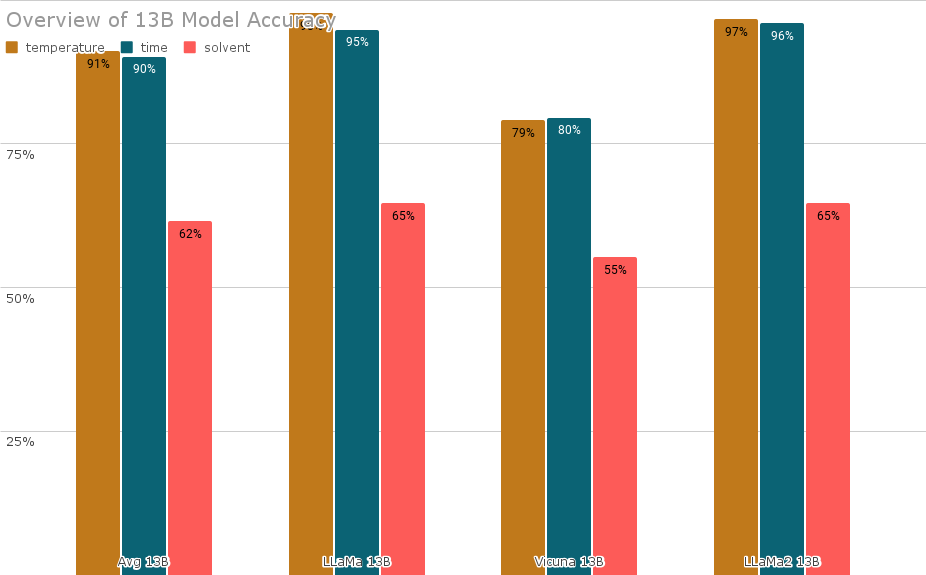
\includegraphics[width=0.9\textwidth]{img/overview_13b_accuracy}
        \caption[Overview of 13B Models Accuracy]{\textbf{Overview of the Accuracy of Models with a Size of 13B parameters.}
        Leftmost is the average over all 13B sized models.
        \model{falcon} does not have a 13B sized variant.
        On average, the accuracy for \ttemp is 90.3\%, 89.1\% for \ttime and 54.4\% for \tsolv.
        }
        \label{fig:13b_acc}
    \end{centering}
\end{figure}


\begin{figure}[!htbp]
    \begin{centering}
        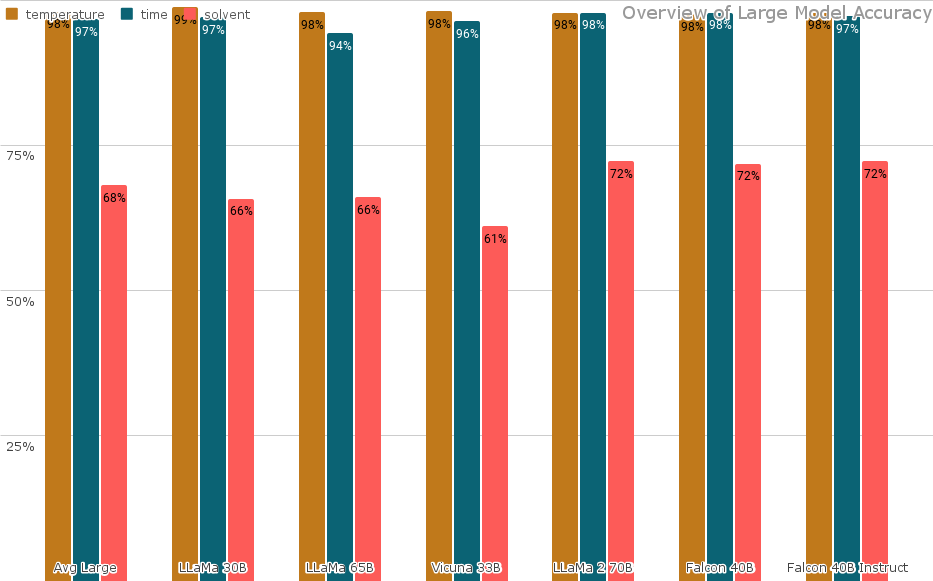
\includegraphics[width=0.9\textwidth]{img/overview_large_accuracy}
        \caption[Overview of Large Model Accuracy]{\textbf{Overview of the Accuracy of Models with a Size over 30B parameters.}
        Leftmost is the average over all models upwards of 30B parameters.
        On average, the accuracy for \ttemp is 98\%, 97\% for \ttime and 68\% for \tsolv.
        \model{llama2} does not have a 30B or 33B-sized variant.
        There is also no \model{vicuna}-65B variant made available from \gls{lmsys}.
        \model{llama2} and both \model{falcon} models achieve 72\% accuracy on \tsolv extraction, 6-11 \glspl{pp} more than other models.
        }
        \label{fig:large_acc}
    \end{centering}
\end{figure}



\section{Accuracy Overview}\label{sec:result:first}

\subsection{7B Parameter Models}\label{sub:result:7b}
As can be seen in \figref{7b_acc}, most models achieve a decent accuracy in extracting \ttemp and \ttime data.
Most models hover a few \glspl{pp} below 60\% in \tsolv accuracy, with \model{vicuna} being an outlier, achieving an accuracy of only 47\%.

\model{llama2} has the highest accuracy for both \ttemp and \ttime, but \model{falcon} is two \glspl{pp} more accurate in \tsolv prediction on our dataset.
Based on this, it seems that \model{llama2}-7B already achieves close to the highest accuracy for extraction of \ttemp, and is close behind on \ttime.


\subsection{13B Parameter Models}\label{sub:result:13b}

As can be seen in \figref{13b_acc}, accuracy improved on average, but primarily for \model{llama}.
In fact, the accuracy of \model{vicuna}-13B even slightly degraded when compared to \model{vicuna}-7B on \ttemp and \ttime, and it mostly stayed stagnant for \model{llama2}.
\model{llama} increased accuracy on \ttemp by 6 \glspl{pp}, but particularly on \ttime by 33 \glspl{pp}. More information on what happened there can be found in \secref{unitconfusion}.

\model{vicuna}-13B is the weakest in accuracy for \ttemp and \ttime, trailing by about 14 \glspl{pp} behind \model{llama} and \model{llama2}. In expecation, \model{falcon}-instruct-13B should still be worse, but \model{falcon} does not have a 13B variant.

\subsection{Large Models}\label{sub:result:large}
See \figref{large_acc}. As much as scores between models differ in \subref{result:7b}, differences between large models are marginal at best. \todo{write results subsection on large models}

\section{Unit Confusion}\label{sec:unitconfusion}
\begin{figure}[!htb]
    \begin{centering}
        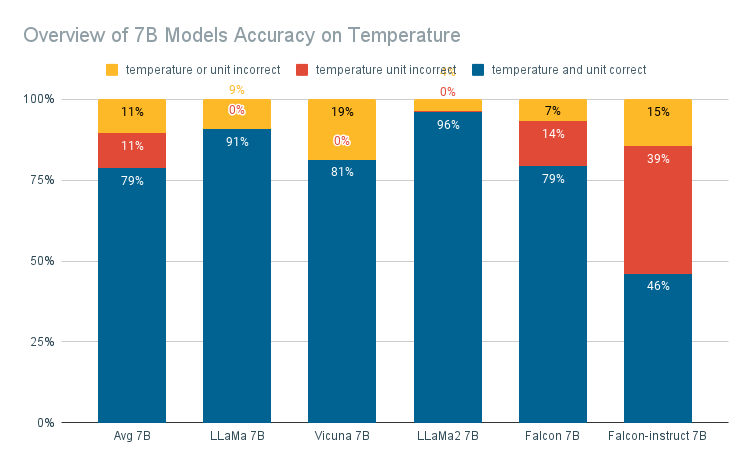
\includegraphics[width=\textwidth]{img/overview_7b_temp}
        \caption[7B Models Detailed Temperature Accuracy]{\textbf{Detailed Overview of 7B Models Accuracy on Temperature.}}
        On average, 7B sized models had an accuracy of 78\% on the extraction of the \ttemp the synthesis was run at.
        Most models did not have problems with temperature units, apart from \model{falcon}.
        \label{fig:7b_temp}
    \end{centering}
\end{figure}

\begin{figure}[!htb]
    \begin{centering}
        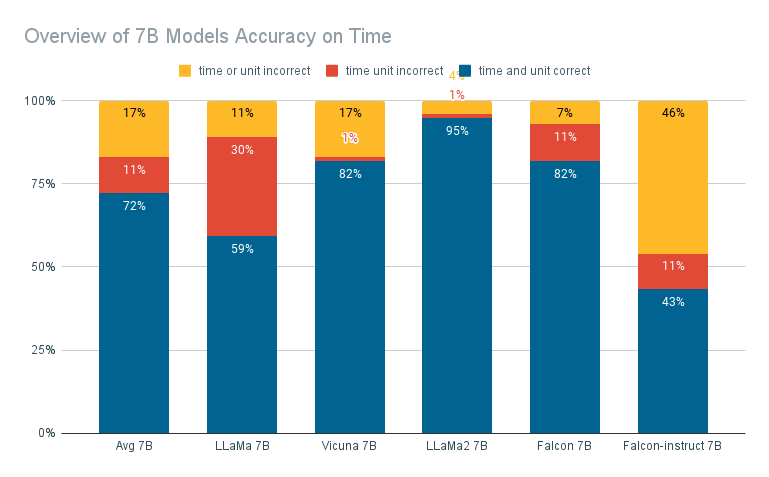
\includegraphics[width=\textwidth]{img/overview_7b_time}
        \caption[7B Models Detailed Time Accuracy]{\textbf{Detailed Overview of 7B Models Accuracy on Time.}
            On average, 7B sized models had an accuracy of 72\% on the extraction of the synthesis duration, and a third of the mistakes (11\% of 28\% total mistakes), were simply due to getting the unit of the duration wrong.
            \model{llama} struggled the most, providing inaccurate units for about a third of all answers on \ttime.
            Both \model{falcon} and \model{falcon}-instruct confused units in about 11\% of answers.
            However, \model{vicuna} and \model{llama2} gave the wrong unit in only 1\% of cases.
        }
        \label{fig:7b_time}
    \end{centering}
\end{figure}

\begin{figure}[!htbp]
    \begin{centering}
        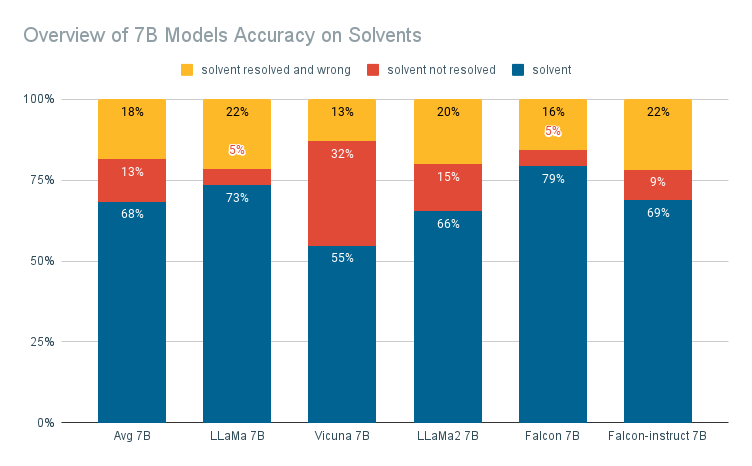
\includegraphics[width=\textwidth]{img/overview_7b_solv}
        \caption[7B Models Detailed Solvent Accuracy]{\textbf{Detailed Overview of 7B Models Accuracy on Solvents.}
            On average, accuracy on \tsolv was 68\%, and an additional 13\% could not be resolved.
            \model{llama}-7B and \model{falcon}-7B had the fewest unresolved answers, at 5\% each.
        }
        \label{fig:7b_solv}
    \end{centering}
\end{figure}

One interesting observation is that smaller models seem to do a lot of 'easy' mistakes.
Not all such simple mistakes can be easily classified, but one certainly can: confusion of units.
\informal{We} counted all instances as \textit{unit confusion}, where the model provided one unit as answer (which was wrong), and \informal{we} could get the correct \ttemp or \ttime only by using a different unit instead.

For example, in one instances \model{falcon} confidently answered 20 °K, when the correct answer would have been 20 °C.

\paragraph{Temperature Units}
As can be seen in \figref{7b_temp}, only \model{falcon} experiences unit confusion for temperature -- and in particular the instruct-variant.
It is unclear why that might be the case exactly, but it seems to be in part of the dataset \model{falcon} was trained on.

\paragraph{Time Units}
Unit confusion on \ttime seems to affect all models to some degree, as can be seen in \figref{7b_time}.
Interestingly, \model{llama} seems to be affected the highest degree, followed by \model{falcon}.


\paragraph{Solvents}\label{par:solv}

\paragraph{Other Mistakes}
When looking through answers manually, \informal{we} discovered additional 'clusters' of mistakes, e.g. adding one too many or too few zeros to \ttime or \ttemp responses.
Smaller models have a higher tendency of making these mistakes, but \informal{we} did not look into these failure modes further due to time constraints.

% (sometimes adding too many or too few zeros, though also often getting it right)

\paragraph{Bigger-sized Models}
Unit confusion on models sized 13B parameters or more is happening in less than 0.5\% of cases (in 0-4 answers of 905 data points).

\todo{build graphs for each model family -- if I have enough time for that}
% \section{Unresolvable Solvents}


\section{Discussion}\label{sec:discussion}
\todo{what does it all mean}
There are two interesting trends \informal{we} can observe across models.

\begin{enumerate}
    \item Larger models are more accurate in the extraction of \ttemp and \ttime.
    \item Accuracy in the extraction of \tsolv is largely the same regardless of model size.
\end{enumerate}

The first one is something \informal{we} would pretty much expect, and it is good to have confirmation of that behaviour.
However, even 13B-sized \model{llama} and \model{llama2} are only marginally worse than any of their bigger siblings, which indicates that even mid-sized models ought to already be fully capable of the extraction of simple parameters such as \ttemp and \ttime.

The second, that \informal{we} see mostly the same accuracy on \tsolv extraction, is indicative of the models getting \textit{confused} rather than fundamentally being incapable of doing it.
The accuracy of just shy of 60\% also indicates that \textit{for the most part} it is clear what the task is.
This suggests that this task could benefit substantially from additional prompt engineering, and maybe even more from fine-tuning. See \secref{out-prompt} and \secref{out-sft} for the outlook on each respectively.


% Some of the answers given are hilarious too \todo{put some example hallucinations in the results chapter}

% \verb!2023-09-09 16:05:36 ERROR    pcp: Could not find `cid` for [distilled H2O]!


\section{Supervised Fine Tuning}\label{sec:sft}
\glspl{LLM} tend to have been pretrained on so much data that they have become generally capable of most tasks even with no fine-tuning \cite{brown_language_2020}.
Fine-tuning a pretrained model instead of a non-pretrained model requires substantially less compute, and sometimes more importantly, hardly any examples to train on to achieve similar results for most tasks \cite{gaddipati_comparative_2020}.

See \secref{training} for more details on pre-training a \gls{LLM} and \subref{finetune} for details on finetunig.

In the end, \informal{we} abandoned fine-tuning due to time constraints. See \secref{con:sft} for conclusions and \secref{out-sft} for an outlook on fine-tuning.

What follows are two excerpts of what \informal{we} encountered when attempting to fine-tune \glspl{LLM} using \gls{transformers}.
While they are by no means exhaustive, other failed approaches followed a similar pattern of wrong or lacking documentation among numerous locally fixed bugs.

\subsection{Excerpt 1: Broken Models}\label{sub:brokenft}
Since \informal{we} have a custom dataset, we also need to write a custom dataloader.
An item of the dataloader can just be the text of the synthesis paragraph -- in a dictionary, as a very specific key.
There is however, only partial and conflicting documentation on the existance and usage of these keys.
\todo{continue writing excerpt 1 from here on}

{
\color{blue}
nuances: tokenization of dataset prior to training. however, which part is doing what?

building custom dataset: array with dicts, with the three required keys \verb`input_ids`, \verb`attention_maska`, and \verb`labels`. curiously, neither is documented particularly well so we tried what is recommended in various tutorials and official sources (e.g. microsoft \cite{deepspeedexamples_2023}):

put the \verb`token_ids` received from tokenization to both \verb`input_ids` and \verb`labels`.

This did result in a model with differing weights than it had before. This model however, was broken as it did not generate anything that was not an EOS-token.
this token is usually used as a stopping criterion during generation.
? resulted in broken model, probably learned that it's 'finished', only outputting EOS tokens. Not sure if doing this otherwise would actually change anything though

Attempts at mask manipulation: not possible with causalLMs (they are all of this type)
}

\subsection{Excerpt 2: Broken Libraries}\label{sub:libraries}
In a later attempt \informal{we} tried using the high-level \gls{hf} \verb`trl` (Transformer Reinforcement Learning) library, which seems to be built for \informal{our} use-case exactly.

{
\color{blue}
However, this library is at best research-grade. The examples, while working with only a few lines, obscure the inner workings of the library.
And good luck: it's also not documented. There is the \verb`DataCollatorForCompletionOnlyLM` collator, which takes a tokenizer, but also doesn't tokenize?!?
\todo{rewrite subsection on broken libraries}

examples only have \verb`text` field, there is a formatting function and whatnot, but this implies tokenization is happening later. nope, errors with 'missing field \verb`token_ids`'.

trying out various things didn't work, until we ultimately didn't have time to continue.

SFT: a lot of magic that isn't documented properly, at all. Couldn't get it to run, gave up due to time limit.
}
% \mintinline{python}{trl} library \cite{hf_trl_supervised}

\todo{add note on additives, detection if one was there in the first place: alternatively outlook}
\todo{explain that we model NER differently, which is why fscore doesn't make sense}


